\documentclass[
]{jss}

%% recommended packages
\usepackage{orcidlink,thumbpdf,lmodern}

\usepackage[utf8]{inputenc}

\author{
Hanne Oberman\\Utrecht University \And Johanna Mu\textasciitilde\{n\}oz
Avila\\University Medical Center Utrecht \AND Valentijn de
Jong\\University Medical Center Utrecht \And Gerko Vink\\Utrecht
University \AND Thomas Debray\\University Medical Center Utrecht
}
\title{Imputation of Incomplete Multilevel Data with \pkg{mice}}

\Plainauthor{Hanne Oberman, Johanna Mu\textasciitilde\{n\}oz
Avila, Valentijn de Jong, Gerko Vink, Thomas Debray}
\Plaintitle{Imputation of Incomplete Multilevel Data with mice}
\Shorttitle{Multilevel \pkg{mice}}


\Abstract{
This is a tutorial paper on imputing incomplete multilevel data with
\pkg{mice}. Footnotes in the current version show work in progress/under
construction. The last section is not part of the manuscript, but purely
for reminders. We aim to submit at JSS, so there is no word count limit
(``There is no page limit, nor a limit on the number of figures or
tables'').
}

\Keywords{missing
data, multilevel, clustering, \pkg{mice}, \proglang{R}}
\Plainkeywords{missing data, multilevel, clustering, mice, R}

%% publication information
%% \Volume{50}
%% \Issue{9}
%% \Month{June}
%% \Year{2012}
%% \Submitdate{}
%% \Acceptdate{2012-06-04}

\Address{
    Hanne Oberman\\
    Utrecht University\\
    Padualaan 14\\
3584 CH Utrecht\\
  E-mail: \email{h.i.oberman@uu.nl}\\
  URL: \url{https://hanneoberman.github.io/}\\~\\
          }


% tightlist command for lists without linebreak
\providecommand{\tightlist}{%
  \setlength{\itemsep}{0pt}\setlength{\parskip}{0pt}}



\usepackage{graphicx}
\usepackage{mathtools}
\usepackage{ulem}

\usepackage{amsmath}

\begin{document}



\hypertarget{introduction}{%
\section{Introduction}\label{introduction}}

\sout{In many contemporary data analysis efforts, some form of
hierarchical or clustered structure is recorded.} Contemporary
decision-making is increasingly often data-driven and sometimes even
entirely dictated by data. Although data relevant for decision makers
were initially collected using small and well-designed studies, there
has been a growing need to address more complex questions at a wider
scale. This not only requires to collect larger amounts of data, but
also from more diverse settings and populations. For example, {[}TD:
introduce IPDMA here; eg. HIV studies Johanna is referring to{]}.
Another example is the use of large databases with information from
thousands or even millions of individuals from multiple cities, regions
or even countries. Finally, a third situation arises when data are
collected from multicenter studies {[}TD: maybe refer to the
schools/classes example here{]}. For example, students may be clustered
in classes in psychometrics research, or patients may be clustered in
studies in individual patient data meta-analyses in medical research. A
common characteristic in aforementioned examples is the presence of
clustering. {[}TD: briefly explain what is clustering?{]}

Ignoring the clustered structure of such multilevel data can be harmful
to the statistical inferences and introduce bias in estimators
\citep{hox17}. \sout{Imagine a case where cross-level interactions
between unit-level variables and cluster-level variables are present.
The cluster to which a unit belongs may then influence the unit-level
observations--and vice versa for each of the units that make up the
cluster.} These relations can and should be taken into account when
developing analysis models for multilevel data for the simple reason
that groups of observations share some common variance. \sout{The
variability due to clustering is often measured by means of the
intraclass coefficient (ICC). The ICC can be seen as the percentage of
variance that can be attributed to the cluster-level, where a high ICC
would indicate that a lot of variability is due to the cluster
structure.} Multilevel models typically accommodate for this variability
by including a separate group mean for each cluster. In addition to
random intercepts, multilevel models can also include random effects and
heterogeneous residual error variances across clusters \citep[see
e.g.][\citet{hox17} and \citet{jong21}]{gelm06}. There are many names
for models that take clustering into account. Some popular examples are
`multilevel models', `hierarchical models', `mixed effect models' and
`random effect models'. {[}TD: emphasize when/why we need to account for
clustering in the analysis of clustered data. Why is the presence of
clustering relevant when considering multiple imputation of missing
data? e.g.~distinction between systematically and sporadically missing
data. But also: mechanisms of missing data (e.g.~MCAR, MAR, MNAR) may
differ between clusters. But also: relation between observed data may
differ between clusters? When/ why should we avoid using traditional
imputation methods? e.g.~congeniality issues.{]}

\hypertarget{missingness-in-multilevel-data}{%
\subsection{Missingness in multilevel
data}\label{missingness-in-multilevel-data}}

\begin{CodeChunk}
\begin{figure}

{\centering 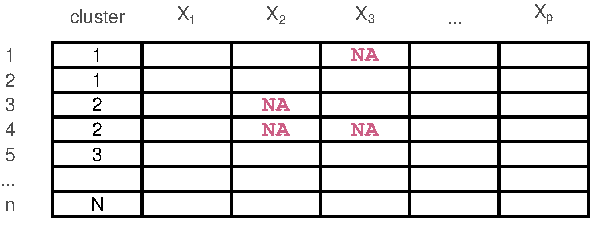
\includegraphics{Imputation_of_Incomplete_Multilevel_Data_files/figure-latex/patterns-1} 

}

\caption[Missingness in multilevel data]{Missingness in multilevel data}\label{fig:patterns}
\end{figure}
\end{CodeChunk}

The process of analyzing multilevel data is further complicated when not
all data entries are observed. Just as with single level data,
missingness may occur at the unit level. But with multiple levels of
data comes the potential for clustered missingness. Therefore,
incomplete multilevel data can be categorized into two general patterns:
systematic missingness and sporadic missingness \citep{resc13}.
Systematic missingness implies that one or more variables are never
observed in a certain cluster. With sporadic missingness there may be
observed data for some but not all units in a cluster
\citep{buur18, jola18}. We have visualized this difference in Figure 1,
which shows an \(n \times p\) set \(\mathbf{X} = X_1, \dots, X_p\), with
\(n\) units distributed over \(N\) clusters, and \(p=3\) columns. Column
\(X1\) is completely observed, column \(X2\) is systematically missing
in cluster 2, and column \(X3\) is sporadically missing. To analyze
these incomplete data, we have to take the nature of the missingness and
the cluster structure into account. For example, the sporadic
missingness in \(X3\) could be easily amended if this would be a
cluster-level variable (and thus constant within clusters). We could
then just extrapolate the true (but missing) value of \(X3\) for unit 1
from unit 2, and the value for unit 4 from unit 3. If \(X3\) would
instead be a unit-level variable (which may vary within clusters), we
could not just recover the unobserved `truth', but would need to use
some kind of missing data method or discard the incomplete units
altogether (i.e., list-wise deletion/complete case analysis). Further,
with the systematic missingness in \(X2\), it is impossible to fit a
multilevel model since we cannot estimate the intercept of cluster 2. We
would have to exclude this cluster from our analyses entirely to obtain
any results. Obviously, excluding observations is not a desirable
workflow.

Ignoring the missingness in analyses can be extremely harmful to
inferences. Complete case analysis can introduce bias in statistical
inferences and lowers statistical power. Instead, the missingness should
be accommodated \emph{before} or \emph{within} the analysis of
scientific interest. Especially the former is very generic and popular.
{[}VJ: add why multiple values are imputed.{]} Imputing (i.e., filling
in) the missing values separates the missing data problem from the
scientific problem: missing data are replaced by plausible values
whereafter the completed data is analyzed as if it were completely
observed. The \proglang{R} package \pkg{mice} has become the de-facto
standard for imputation by chained equations, which iteratively solves
the missingness on a variable-by-variable basis. \pkg{mice} is known to
yield valid inferences under many different missing data circumstances
\citep{buur18}. In this paper, we will discuss how to use \pkg{mice} in
the context of multilevel data.

\hypertarget{aim-of-this-paper}{%
\subsection{Aim of this paper}\label{aim-of-this-paper}}

This papers serves as a tutorial for imputing incomplete multilevel data
with \pkg{mice}. We provide practical guidelines and code snippets for
different missing data situations, including missing not at random
(MNAR) mechanisms \citep[where the probability to be missing depends on
unrecorded information, making the missingness
non-ignorable,][]{rubi76, meng94}. For reasons of brevity, we focus on
imputation by chained equations wit \pkg{mice} exclusively\footnote{Note
  that the alternative, joint modeling imputation for multilevel data or
  \pkg{jomo} \citet{jomo}, has been implemented in \pkg{mice} as well
  but is outside the scope of this tutorial.}. Other useful resources
for the analysis of incomplete multilevel data include the \proglang{R}
packages \pkg{mitml}, \pkg{miceadds}, and \pkg{mdmb}, and empirical work
by \citet{audi18} and \citet{grun18}. Please note that this tutorial
paper assumes a basic level of knowledge on multilevel
models.\footnote{Note to self: We're providing an overview of
  implementations. It's up-to the reader to decide which multilevel
  strategy suits their data. We won't go into detail for the different
  methods (and equations). This paper is just a software tutorial, so
  we'll keep it practical.} Assumed knowledge also includes the use of
the `piping operator', \texttt{\%\textgreater{}\%}, adopted from the
\pkg{magrittr} package, and the \pkg{lme4} notation for multilevel
models.\footnote{TODO: Add environment info, seed and version number(s)
  somewhere!}

We illustrate how to impute incomplete multilevel data by means of three
case studies:

\begin{itemize}
\tightlist
\item
  \texttt{popmis} from the \pkg{mice} package \citep[simulated data on
  perceived popularity, \(n = 2,000\) pupils across \(N = 100\)
  schools,][]{mice};
\item
  \texttt{hiv} from the \pkg{GJRM} package \citep[simulated data on HIV
  diagnoses, \(n = 6,416\) patients across \(N = 9\) regions,][]{GJRM};
\item
  \texttt{impact} from the \pkg{metamisc} package \citep[empirical data
  on traumatic brain injuries, \(n = 11,022\) patients across \(N = 15\)
  studies,][]{metamisc}.
\end{itemize}

For each of these datasets, we will discuss the nature of the
missingness, choose one or more imputation models and evaluate the
imputed data, but we will also highlight one specific aspect of the
imputation workflow. With the \texttt{popmis} data, we show how (and how
not) to develop an imputation model. With the \texttt{hiv} data we focus
on extending the imputation model to include Heckman-type
selection-inclusion methods. With the \texttt{impact} data we provide an
example of multivariate missingness in real-world data. Together, this
should give enough scaffolding for applied researchers who are faced
with incomplete multilevel data.\footnote{TODO: Add notation paragraph
  or `translation table' linking multilevel equations to \pkg{lme4}
  formulas. Use betas instead of gamma's and mu's. Add interpretation of
  values in predictormatrix (-2 for the cluster variable, 2 for random
  effects). Add ICC and congeneality here as well. And make missingness
  mechanism table as well.}

Set-up the R environment and load the necessary packages:

\begin{CodeChunk}
\begin{CodeInput}
R> set.seed(2022)
R> library(mice)
R> library(ggmice)
R> library(ggplot2)
R> library(dplyr)
R> library(lme4)
R> library(mitml)
\end{CodeInput}
\end{CodeChunk}

\begin{center}\rule{0.5\linewidth}{0.5pt}\end{center}

\begin{center}
REVIEW UNTIL THIS POINT SVP
\end{center}

\begin{center}\rule{0.5\linewidth}{0.5pt}\end{center}

\hypertarget{case-study-i-how-not-to-impute}{%
\section{Case Study I: How (not) to
impute}\label{case-study-i-how-not-to-impute}}

In this section we'll go over the different steps involved with imputing
incomplete multilevel data. The data we're using is the \texttt{popmis}
dataset from the \texttt{mice} package. This is a simulated dataset with
pupils (\(n = 2000\)) clustered within schools (\(N = 100\)). In this
tutorial we'll use the following variables:

\begin{itemize}
\tightlist
\item
  \texttt{school}, school identification number (clustering variable);
\item
  \texttt{popular}, pupil popularity (self-rating between 0 and 10;
  unit-level);
\item
  \texttt{sex}, pupil sex (0=boy, 1=girl; unit-level);
\item
  \texttt{texp}, teacher experience (in years; cluster-level).
\end{itemize}

The analysis model corresponding to this dataset is multilevel
regression with random intercepts, random slopes and a cross-level
interaction. The outcome variable is \texttt{popular}, which is
predicted from the unit-level variable \texttt{sex} and the
cluster-level variable \texttt{texp}. The regression equation\footnote{add
  the `level notation' (Bryk and Raudenbush, 1992) and/or matrix
  notation (`linear mixed effects model'; Laird and Ware, 1982) too?}
and \texttt{lme4} notation for this model are

\[
\text{popular}_{ij} =
\gamma_{00} + 
\gamma_{10} \text{ sex}_{ij} + 
\gamma_{01} \text{ texp}_{j} + 
\gamma_{11} \text{ texp}_{j} \times \text{sex}_{ij} + 
u_{0j} + 
u_{1j} \text{ sex}_{ij} + 
e_{ij} \\
\]

\[
\texttt{popular} \sim  \texttt{1 + sex + texp + sex:texp + (1 + sex | school)}
\]

Since the data is simulated and the missingness is induced, we can
compare our inferences after imputation to the true complete data. The
data is created in such a way that the clustering variable
\texttt{school} explains quite some variance in the outcome variable
\texttt{popular}. We express this using the intraclass correlation, ICC
\(=\) 0.58. We'll evaluate the ICC after each missing data strategy, and
compare the estimated fixed effects:

\begin{CodeChunk}
\begin{CodeOutput}
                 Estimate with 95% CI
1 (Intercept)  3.314 [ 2.998,  3.629]
2         sex  1.330 [ 1.069,  1.590]
3        texp  0.110 [ 0.090,  0.130]
4    sex:texp -0.034 [-0.051, -0.017]
\end{CodeOutput}
\end{CodeChunk}

\hypertarget{incomplete-data}{%
\subsubsection{Incomplete data}\label{incomplete-data}}

Load the data into the environment and select the relevant variables:

\begin{CodeChunk}
\begin{CodeInput}
R> popmis <- popmis[, c("school", "popular", "sex", "texp")] 
\end{CodeInput}
\end{CodeChunk}

Plot the missing data pattern:

\begin{CodeChunk}
\begin{CodeInput}
R> plot_pattern(popmis)
\end{CodeInput}
\begin{figure}

{\centering 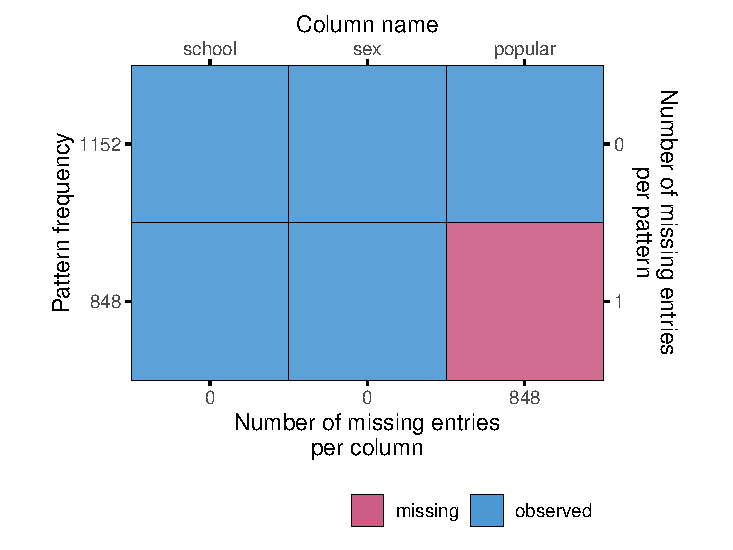
\includegraphics{Imputation_of_Incomplete_Multilevel_Data_files/figure-latex/pop_pat-1} 

}

\caption[Missing data pattern in the popularity data]{Missing data pattern in the popularity data}\label{fig:pop_pat}
\end{figure}
\end{CodeChunk}

The missingness is univariate and sporadic, which is illustrated in the
missing data pattern in Figure \ref{fig:pop_pat}. The ICC in the
incomplete data is 0.56. This tells us that the multilevel structure of
the data should probably be taken into account. If we don't, we'll may
end up with incorrect imputations, biasing the effect of the clusters
towards zero.

Plot the correlations in the incomplete data:

\begin{CodeChunk}
\begin{CodeInput}
R> plot_corr(popmis)
\end{CodeInput}


\begin{center}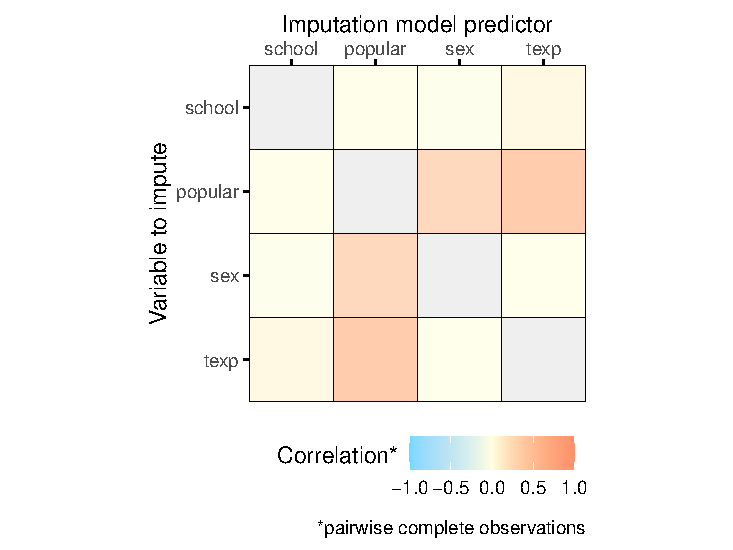
\includegraphics{Imputation_of_Incomplete_Multilevel_Data_files/figure-latex/pop-corr-1} \end{center}

\end{CodeChunk}

To develop the best imputation model for the incomplete variable
\texttt{popular}, we need to know whether the missingness depends on the
observed values of other variables. We'll highlight one other variable
to illustrate, but ideally one would inspect all relations. The
questions we'll ask are: `Does the missing data of pupil popularity
(\texttt{popular}) depend on observed teacher popularity
(\texttt{texp})?'. This can be evaluated statistically, but visual
inspection usually suffices. We'll make a histogram of \texttt{texp}
separately for the pupils with known popularity and missing popularity.

Plot the histogram for teacher experience conditional on the missingness
indicator of \texttt{popular}:

\begin{CodeChunk}
\begin{CodeInput}
R> ggmice(popmis, aes(texp)) +
+   geom_histogram(fill = "white") +
+   facet_grid(. ~ is.na(popular), labeller = label_both)
\end{CodeInput}


\begin{center}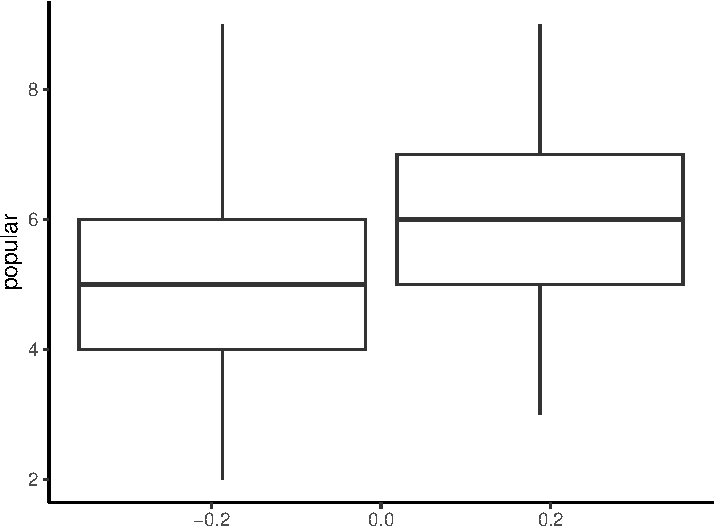
\includegraphics{Imputation_of_Incomplete_Multilevel_Data_files/figure-latex/pop-hist-1} \end{center}

\end{CodeChunk}

TODO: think about what is a meaningful rule of thumb to signal that the
user should be worried?

This shows us that there are no apparent differences in the distribution
of \texttt{texp} depending on the missingness indicator of
\texttt{popular} (t = -0.873, p = 0.383).

\hypertarget{complete-case-analysis-not-recommended}{%
\subsubsection{Complete case analysis (not
recommended)}\label{complete-case-analysis-not-recommended}}

Complete case analysis ignores the observations with missingness
altogether, which lowers statistical power and may even introduce bias
in MCAR situations.

\hypertarget{imputation-ignoring-the-cluster-variable-not-recommended}{%
\subsubsection{Imputation ignoring the cluster variable (not
recommended)}\label{imputation-ignoring-the-cluster-variable-not-recommended}}

The first imputation model that we'll use is likely to be invalid. We do
\emph{not} use the cluster identifier \texttt{school} as imputation
model predictor. With this model, we ignore the multilevel structure of
the data, despite the high ICC. This assumes exchangeability between
units. We include it purely to illustrate the effects of ignoring the
clustering in our imputation effort. We'll use the default imputation
methods in \texttt{mice()} (predictive mean matching to impute the
continuous variables and logistic regression to impute binary
variables).

Create a methods vector and predictor matrix for \texttt{popular}, and
make sure \texttt{school} is not included as predictor:

\begin{CodeChunk}
\begin{CodeInput}
R> meth <- make.method(popmis) # methods vector
R> pred <- quickpred(popmis)   # predictor matrix
R> plot_pred(pred)
\end{CodeInput}


\begin{center}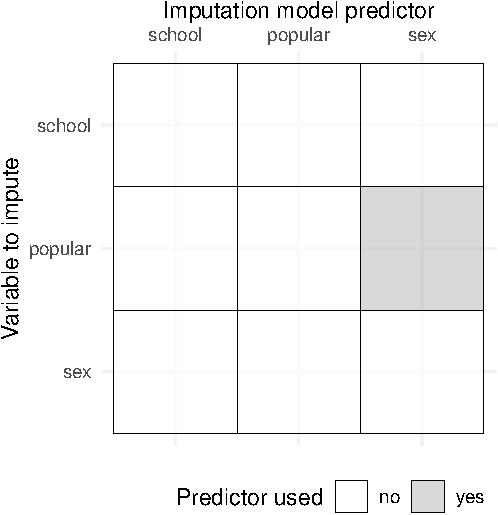
\includegraphics{Imputation_of_Incomplete_Multilevel_Data_files/figure-latex/pop-ignored-pred-1} \end{center}

\end{CodeChunk}

Impute the data, ignoring the cluster structure:

\begin{CodeChunk}
\begin{CodeInput}
R> imp_ignored <- mice(popmis, maxit = 1, pred = pred, print = FALSE)
\end{CodeInput}
\end{CodeChunk}

TODO: remove the broom.mixed output, use mitml only

Analyze the imputations:

\begin{CodeChunk}
\begin{CodeInput}
R> fit_ignored <- imp_ignored %>% 
+   with(lme4::lmer(popular ~ 1 + sex + texp + sex:texp + (1 + sex | school))) 
R> testEstimates(as.mitml.result(fit_ignored), var.comp = TRUE)
\end{CodeInput}
\begin{CodeOutput}

Call:

testEstimates(model = as.mitml.result(fit_ignored), var.comp = TRUE)

Final parameter estimates and inferences obtained from 5 imputed data sets.

             Estimate Std.Error   t.value        df   P(>|t|)       RIV       FMI 
(Intercept)     3.354     0.245    13.704     6.831     0.000     3.260     0.813 
sex             1.247     0.332     3.759     6.154     0.009     4.160     0.849 
texp            0.110     0.017     6.320     6.084     0.001     4.286     0.852 
sex:texp       -0.027     0.022    -1.225     5.914     0.267     4.631     0.862 

                            Estimate 
Intercept~~Intercept|school    0.177 
sex~~sex|school                0.232 
Intercept~~sex|school         -0.043 
Residual~~Residual             0.670 
ICC|school                     0.209 

Unadjusted hypothesis test as appropriate in larger samples.
\end{CodeOutput}
\end{CodeChunk}

\begin{CodeChunk}


\begin{center}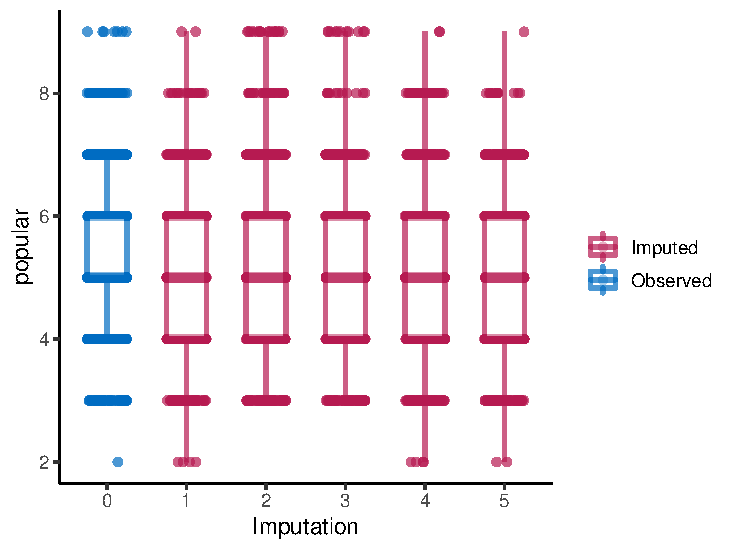
\includegraphics{Imputation_of_Incomplete_Multilevel_Data_files/figure-latex/pop_ignored_eval-1} \end{center}

\end{CodeChunk}

\hypertarget{imputation-with-the-cluster-variable-as-predictor-not-recommended}{%
\subsubsection{Imputation with the cluster variable as predictor (not
recommended)}\label{imputation-with-the-cluster-variable-as-predictor-not-recommended}}

We'll now use \texttt{school} as a predictor to impute all other
variables. This is still not recommended practice, since it only works
under certain circumstances and results may be biased
\citep{drec15, ende16}. But at least, it includes some multilevel
aspect. This method is also called `fixed cluster imputation', and uses
N-1 indicator variables representing allocation of N clusters as a fixed
factor in the model \citep{reit06, ende16}. Colloquially, this is
`multilevel imputation for dummies'.

Add: doesn't work with syst missing (only sporadically). There's some
pro's and con's. May not differ much if the number of clusters is low.

The more the random effects are of interest, the more you need ml
models.

\begin{CodeChunk}
\begin{CodeInput}
R> # adjust the predictor matrix
R> pred["popular", "school"] <- 1 
R> plot_pred(pred)
\end{CodeInput}


\begin{center}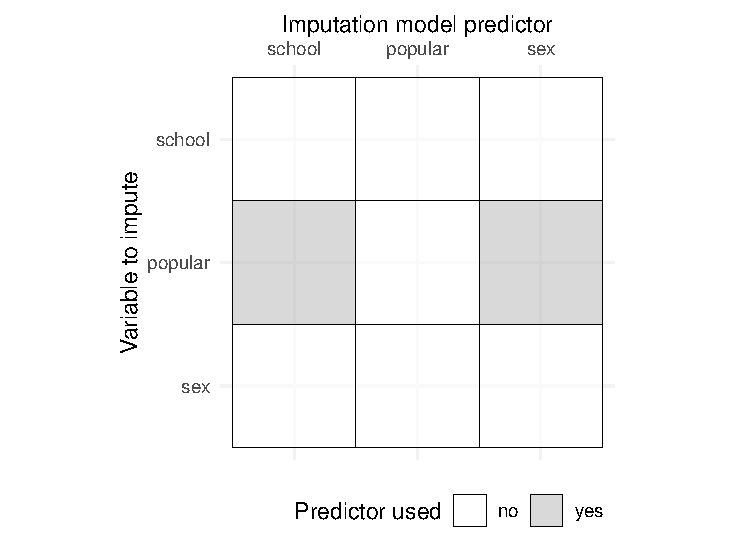
\includegraphics{Imputation_of_Incomplete_Multilevel_Data_files/figure-latex/pop_predictor-1} \end{center}

\begin{CodeInput}
R> # impute the data, cluster as predictor
R> imp_predictor <- mice(popmis, maxit = 1, pred = pred, print = FALSE)
\end{CodeInput}
\end{CodeChunk}

\begin{CodeChunk}


\begin{center}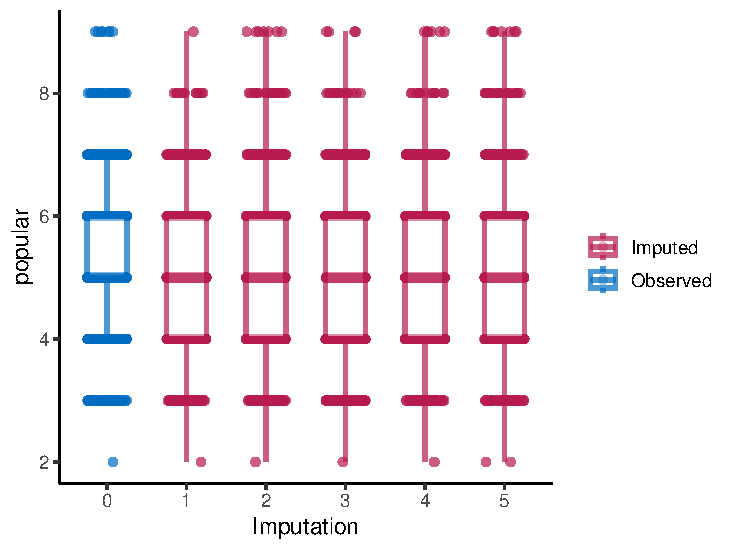
\includegraphics{Imputation_of_Incomplete_Multilevel_Data_files/figure-latex/pop_predictor_eval-1} \end{center}

\end{CodeChunk}

Now, we can clearly see that the imputed values of \texttt{texp} are
higher than the observed values, which is in line with right-tailed MAR.

The ICCs are way more in line with the ICCs in the incomplete data. But
this is a quick and dirty way of imputing multilevel data. We
\emph{should} be using a multilevel model.

\hypertarget{imputation-with-random-effects}{%
\subsubsection{Imputation with random
effects}\label{imputation-with-random-effects}}

With \texttt{2l.norm} we impute the outcome with a multilevel model
assuming random slopes for each variable in the imputation model and
homogeneous within-cluster variance.

``Van Buuren (2011) considered the homoscedastic linear mixed model as
invalid for imputing incomplete predictors, and investigated only the
2l.norm method, which allows for heterogeneous error variances''
\citep{buur18}.

\begin{CodeChunk}
\begin{CodeInput}
R> # adjust the predictor matrix
R> pred["popular", ] <- c(school = -2, popular = 0, sex = 2, texp = 2) 
R> plot_pred(pred) 
\end{CodeInput}


\begin{center}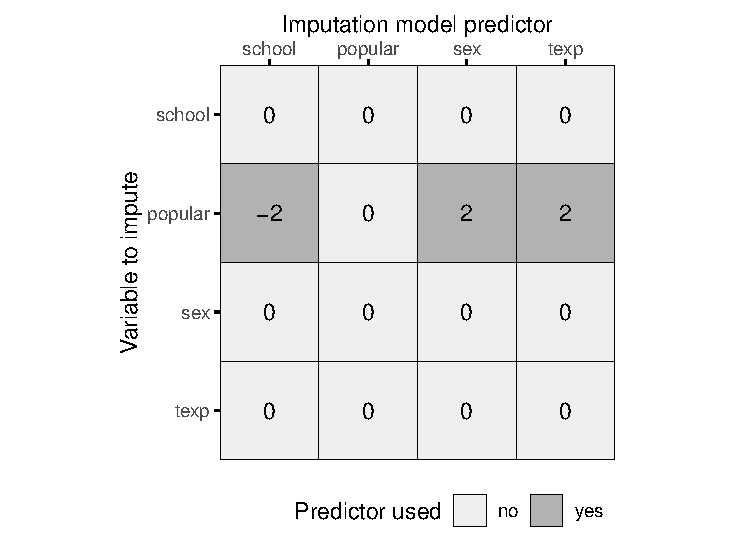
\includegraphics{Imputation_of_Incomplete_Multilevel_Data_files/figure-latex/pop_norm-1} \end{center}

\begin{CodeInput}
R> meth <- make.method(popmis)
R> meth["popular"] <- "2l.pmm"
R> imp_pmm_2l <-
+   mice(
+     popmis %>% mutate(school = as.integer(school)),
+     pred = pred,
+     meth = meth,
+     maxit = 1,
+     print = FALSE
+   )
\end{CodeInput}
\end{CodeChunk}

\begin{CodeChunk}


\begin{center}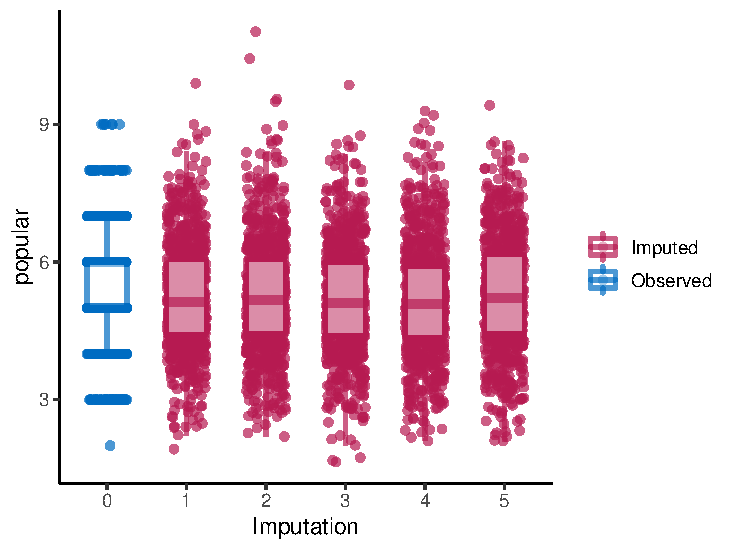
\includegraphics{Imputation_of_Incomplete_Multilevel_Data_files/figure-latex/pop_norm_eval-1} \end{center}

\end{CodeChunk}

\hypertarget{imputation-with-random-effects-and-heterogeneity}{%
\subsubsection{Imputation with random effects and
heterogeneity}\label{imputation-with-random-effects-and-heterogeneity}}

This method assumes random slopes for each variable in the imputation
model. In contrast to \texttt{2l.norm} this method allows a
cluster-specific residual error variance.

\begin{CodeChunk}
\begin{CodeInput}
R> pred["popular", ] <- c(-2, 2, 1, 2)
R> meth <- c("", "2l.pan", "", "")
R> imp_pan_2l <-
+   mice(
+     popmis %>% mutate(school = as.integer(school)),
+     pred = pred,
+     meth = meth,
+     maxit = 1,
+     print = FALSE
+   )
\end{CodeInput}
\end{CodeChunk}

\begin{CodeChunk}


\begin{center}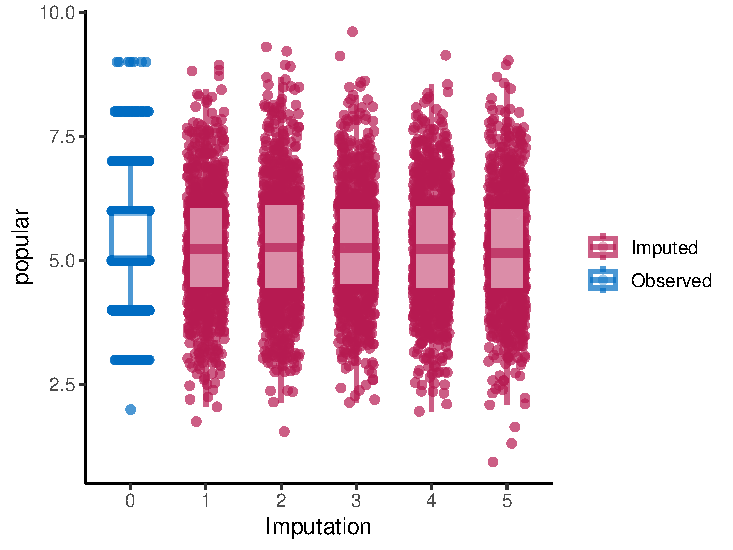
\includegraphics{Imputation_of_Incomplete_Multilevel_Data_files/figure-latex/pop_pan_eval-1} \end{center}

\end{CodeChunk}

\hypertarget{how-to-handle-non-random-selection-case-study-ii-hiv}{%
\section{How to handle non-random selection (Case study II:
HIV)}\label{how-to-handle-non-random-selection-case-study-ii-hiv}}

Data are simulated and included in the \texttt{GJRM} package. We will
use the following variables:

\begin{itemize}
\tightlist
\item
  \texttt{region} Cluster variable,
\item
  \texttt{hiv} HIV diagnosis (0=no, 1=yes),
\item
  \texttt{age} Age of the patient,
\item
  \texttt{marital} Marital status,
\item
  \texttt{condom} Condom use during last intercourse,
\item
  \texttt{smoke} Smoker (levels; inclusion restriction variable).
\end{itemize}

The imputation of these date is based on the toy example from
\href{https://github.com/johamunoz/Heckman-IPDMA/blob/main/Toy_example.R}{IPDMA
Heckman Github repo}.

\begin{CodeChunk}


\begin{center}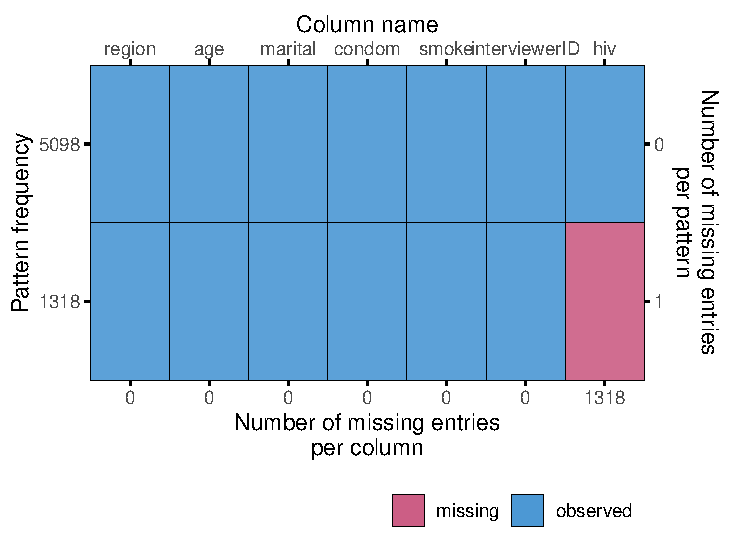
\includegraphics{Imputation_of_Incomplete_Multilevel_Data_files/figure-latex/hiv-1} \end{center}

\end{CodeChunk}

From the missing data pattern we see that we can set \texttt{maxit} to
1, since there is only one variable with missingness.

The inclusion restriction variable should be a predictor of the the
actual value of the variable of interest, but \emph{not} of missingness
indicator for the variable of interest. In this case, the data were
simulated to adhere to this requirement. Namely, \(\beta_{smoke}\) =
-0.064, 95\% CI {[}-0.256, 0.126{]} for the analysis model
(\texttt{formula\ =\ hiv\ \textasciitilde{}\ .}), and \(\beta_{smoke}\)
= -0.265, 95\% CI {[}-0.422, -0.11{]} for the selection model
(\texttt{formula\ =\ is.na(hiv)\ \textasciitilde{}\ .}). This means the
assumptions for the Heckman-type selection model are met.

\hypertarget{how-to-handle-multivariate-missingness-case-study-iii-impact}{%
\section{How to handle multivariate missingness (Case study III:
IMPACT)}\label{how-to-handle-multivariate-missingness-case-study-iii-impact}}

\texttt{impact} is traumatic brain injury data with patients,
\(n = 11022\), clustered in studies, \(N = 15\). With the following 11
variables:

\begin{itemize}
\tightlist
\item
  \texttt{name} Name of the study,
\item
  \texttt{type} Type of study (RCT: randomized controlled trial, OBS:
  observational cohort),
\item
  \texttt{age} Age of the patient,
\item
  \texttt{motor\_score} Glasgow Coma Scale motor score,
\item
  \texttt{pupil} Pupillary reactivity,
\item
  \texttt{ct} Marshall Computerized Tomography classification,
\item
  \texttt{hypox} Hypoxia (0=no, 1=yes),
\item
  \texttt{hypots} Hypotension (0=no, 1=yes),
\item
  \texttt{tsah} Traumatic subarachnoid hemorrhage (0=no, 1=yes),
\item
  \texttt{edh} Epidural hematoma (0=no, 1=yes),
\item
  \texttt{mort} 6-month mortality (0=alive, 1=dead).
\end{itemize}

The analysis model for this dataset is a prediction model with
\texttt{mort} as the outcome.\footnote{Look at analysis model, maybe
  copy from GREAT data example e.g., adjusted prognostic effect of
  \texttt{ct} on unfortunate outcomes, we just want to know the adjusted
  odds ratio for \texttt{ct}. Add something about systematically missing
  data here.} The data is already imputed (Steyerberg et al, 2008), so
we've induced missingness again based on the missingness in the original
data.

\[
\text{mort}_{ij} =
\gamma_{00} + 
\gamma_{01} \text{ type}_{j} + 
\gamma_{10} \text{ age}_{ij} + 
\gamma_{10} \text{ moter\_score}_{ij} + 
\gamma_{10} \text{ pupil}_{ij} + 
\gamma_{10} \text{ ct}_{ij} + \\
u_{0j} + 
u_{1j} \text{ age}_{ij} + 
u_{1j} \text{ moter\_score}_{ij} +  
u_{1j} \text{ pupil}_{ij} +  
u_{1j} \text{ ct}_{ij} +  
e_{ij} \\
\]

\texttt{glmer(mort\ \textasciitilde{}\ 1\ +\ type\ +\ age\ +\ motor\_score\ +\ pupil\ +\ ct\ +\ (1\ \textbar{}\ name))}

\begin{CodeChunk}


\begin{center}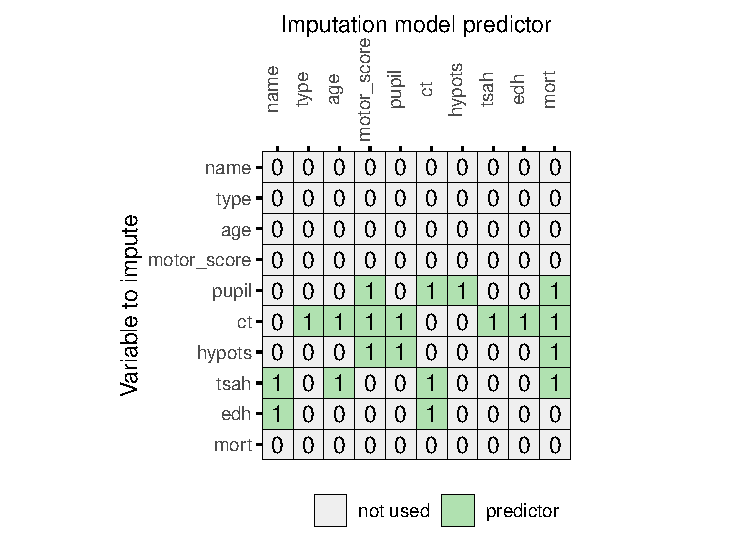
\includegraphics{Imputation_of_Incomplete_Multilevel_Data_files/figure-latex/impact-1} \end{center}

\end{CodeChunk}

\begin{CodeChunk}


\begin{center}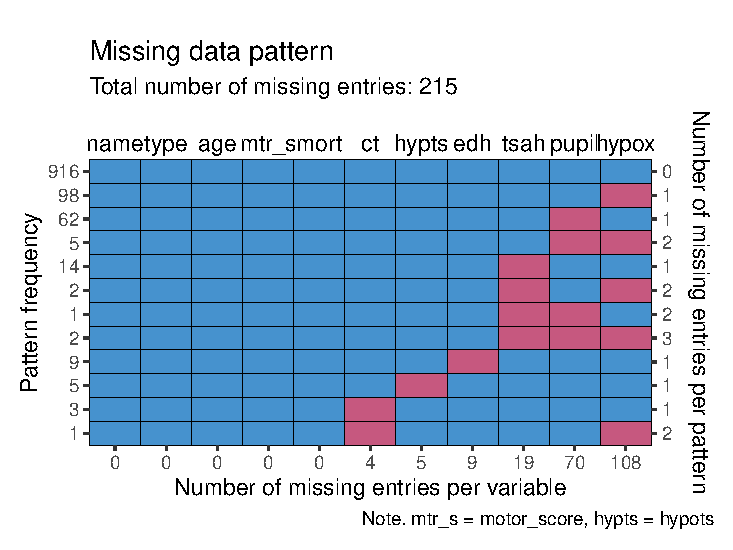
\includegraphics{Imputation_of_Incomplete_Multilevel_Data_files/figure-latex/impact_md-1} \end{center}



\begin{center}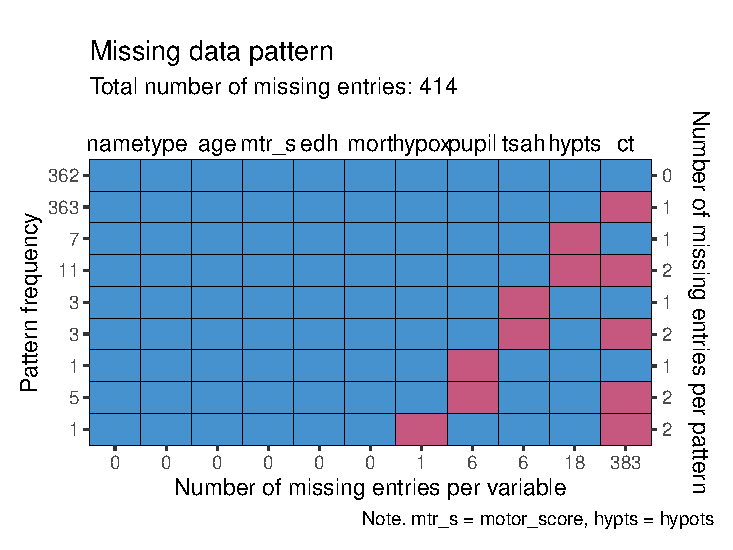
\includegraphics{Imputation_of_Incomplete_Multilevel_Data_files/figure-latex/impact_md-2} \end{center}

\end{CodeChunk}

\begin{CodeChunk}
\begin{CodeOutput}
# A tibble: 22 x 5
   term                 estimate std.error statistic  p.value
   <chr>                   <dbl>     <dbl>     <dbl>    <dbl>
 1 (Intercept)           -3.37     0.205     -16.4   1.97e-60
 2 typeRCT                0.395    0.177       2.23  2.59e- 2
 3 age                    0.0301   0.00191    15.8   5.01e-56
 4 motor_score3          -0.618    0.0829     -7.45  9.33e-14
 5 motor_score4          -1.00     0.0850    -11.8   6.07e-32
 6 motor_score5/6        -1.53     0.0874    -17.5   7.92e-69
 7 pupil                  0.434    0.0398     10.9   9.36e-28
 8 ct                     0.428    0.0344     12.4   1.50e-35
 9 as.factor(name)CSTAT  -0.177    0.199      -0.892 3.72e- 1
10 as.factor(name)EBIC    0.560    0.174       3.22  1.30e- 3
# ... with 12 more rows
\end{CodeOutput}
\end{CodeChunk}

If we run the multilevel model on the incomplete date, we get a warning
about unindentifyability. This means that with CCA as missing data
method, we cannot trust the estimates. To still obtain some estimates to
compare later, we fit a simplified analysis model: using the cluster
variable as indicator in the model.

\begin{CodeChunk}
\begin{CodeInput}
R> pred <- quickpred(impact_NA)
R> pred[pred == 1] <- 2
R> pred[, "name"] <- -2
R> pred["mort", ] <- 2
R> pred[, "mort"] <- 2
R> diag(pred) <- 0
R> pred[c("name", "type", "age", "motor_score", "mort"), ] <- 0
R> pred
\end{CodeInput}
\begin{CodeOutput}
            name type age motor_score pupil ct hypox hypots tsah edh mort
name           0    0   0           0     0  0     0      0    0   0    0
type           0    0   0           0     0  0     0      0    0   0    0
age            0    0   0           0     0  0     0      0    0   0    0
motor_score    0    0   0           0     0  0     0      0    0   0    0
pupil         -2    0   0           2     0  2     0      2    0   0    2
ct            -2    2   2           2     2  0     0      0    2   2    2
hypox         -2    2   0           2     0  0     0      2    0   0    2
hypots        -2    0   0           2     2  0     2      0    0   0    2
tsah          -2    0   2           0     0  2     0      0    0   0    2
edh           -2    0   0           0     0  2     0      0    0   0    2
mort           0    0   0           0     0  0     0      0    0   0    0
\end{CodeOutput}
\begin{CodeInput}
R> meth <- make.method(impact_NA)
R> meth[meth != ""] <- "2l.pmm"
\end{CodeInput}
\end{CodeChunk}

\begin{CodeChunk}
\begin{CodeInput}
R> # imp_impact <- impact_NA %>%
R> #   mutate(name = as.integer(name), motor_score = as.numeric(motor_score)) %>%
R> #   mice::mice(., m = 2, maxit = 1, method = meth, predictorMatrix = pred)
R> # look at jomo for categorical variables?
R> # semi-cont with jomo is not ideal (schafer, '97) because you need 2-step approach
R> # pmm is better (more efficient) because it will still look for donors (maybe outside of cluster) based on predictive distance, even for very small clusters
R> # make assumptions of these methods explicit!
\end{CodeInput}
\end{CodeChunk}

\hypertarget{discussion}{%
\section{Discussion}\label{discussion}}

\begin{itemize}
\item
  JOMO in \pkg{mice} -\textgreater{} on the side for now
\item
  Additional levels of clustering
\item
  More complex data types: timeseries and polynomial relationship in the
  clustering.
\end{itemize}

\hypertarget{think-about}{%
\section{Think about}\label{think-about}}

\begin{itemize}
\item
  Adding some kind of help function to mice that suggests a suitable
  predictor matrix to the user, given a certain analysis model.
\item
  Adding a \texttt{multilevel\_ampute()} wrapper function in mice.
\item
  Exporting \texttt{mids} objects to other packages like \texttt{lme4}
  or \texttt{coxme}?
\item
  Adding a ICC=0 dataset to show that even if there is no clustering it
  doesn't hurt.
\item
  Show use case for deductive imputation for cluster level variables?
\item
  env dump in repo
\end{itemize}

\renewcommand\refname{References}
\bibliography{../References/multilevelmice.bib}



\end{document}
